\documentclass[conference,compsoc]{IEEEtran}
% *** CITATION PACKAGES ***
%
\ifCLASSOPTIONcompsoc
  \usepackage[nocompress]{cite}
\else
  % normal IEEE
  \usepackage{cite}
\fi
% *** GRAPHICS RELATED PACKAGES ***
\usepackage{graphicx} % support the \includegraphics command and options
% *** MATH PACKAGES ***
\usepackage{amsmath}
% *** PDF, URL AND HYPERLINK PACKAGES ***
%
%\usepackage{url}

%%%%%%%%%%%%%%%%%%%%%%%%%%%%%%%%%%%%%%%%%%%%%%%%%%%%%%%%%%%%%%%%%%%%%%%%%%%%%%%%%%%%%%%%%%%%%%%%%%%%%%%%%%%%%%

\begin{document}

\IEEEoverridecommandlockouts
\IEEEpubid{0000--0000/00\$00.00˜\copyright˜2018 Itzel Tapia \& Michael Dominguez} 

\title{Security and Privacy in Connected Autonomous Cars}

\author{\IEEEauthorblockN{Itzel Ramirez Tapia}
\IEEEauthorblockA{University of Texas at Dallas\\Department of Computer Science\\
Email: irt170001@utdallas.edu}
\and
\IEEEauthorblockN{Michael Dominguez}
\IEEEauthorblockA{Sam Houston State University\\Department of Computer Science\\
Email: mad061@shsu.edu}}
\thispagestyle{plain}
\pagestyle{plain}

\maketitle


\begin{abstract}
Technology and infrastructure is currently being researched and developed to support fully autonomous, connected cars. This work includes developing an environment in which these vehicles will have the ability to communicate with each other. This, however, exposes the autonomous system to new vulnerabilities, such as malicious attacks and abuse of privacy. This paper will explain the fundamentals of secure communication, requirements for a network to be considered secure, types of security that exist today, and then propose a cryptographic protocol through which secure communication in connected autonomous cars can be achieved. Connected technology will inherently produce frequent transmissions and sensitive information will be handled. This requires attention be given to define, uphold, and develop necessary privacy standards and protocols. This process has not yet begun, and therefore this paper will also serve to point out important privacy requirements which must be paired with explicit protocols. The important requirements of secure and private communication in connected vehicles will be analyzed, along with possible ways these requirements can be achieved, what current measures are in use, and ways to improve them.  
\end{abstract}


\section{Introduction}
Operating a vehicle is the single most dangerous activity people, both routinely and willingly, engage in. A great part of the risk associated with driving can be attributed to the human factor, i.e. drunk driving, poor visibility, etc., so this then begins to elucidate what measures must be taken. This is a contributing factor and has greatly motivated the development and research of Intelligent Transportation Systems (ITS). Self-driving cars are considered safer than human-operated vehicles. Although many are reluctant to relinquish control of their cars [8], current studies indicate autonomous vehicles will greatly improve traffic flow and have the potential to reduce traffic accidents, particularly those that are attributed to irresponsible human behavior [17]. 

The recent development of autonomous vehicle technology has been a cause for debate. It also raises questions as to how people will interact with ITS [17]. This technology, however, is not unprecedented. The beginning of the autopilot can be traced as far back as 1914 when Lawrence B. Sperry “introduced the first gyroscopic Airplane Stabilizer” [17]. Automated airplanes have been operational both commercially and in military applications. Future applications of ITS will inevitably infiltrate roadways, and several companies and universities are in the testing stages of developing this technology [22].  

The functionality of a vehicle can be categorized into two basic types of functions, safety critical and non-safety critical functions. Safety critical functions include collision warning, emergency broadcast, roadside assistance, emergency response, and vehicle preferences.  Non-safety critical functions include changing lanes, breaking, accelerating, platooning\footnote {Platooning happens when cars hook “themselves to another group of cars heading in the same direction” [23]. They maintain a set distance from each other and follow the same path.}, and route change. This distinction is important, specifically when addressing security concerns, because some of the ITS requirements are more safety-critical than others and as such the information transmitted will need to be kept secure and private.

\subsection{Key Terms}
For clarity, we will define key terms and concepts that will be discussed in this paper. Some terms have been used interchangeably in the past, and this has been a cause for confusion or has left some concepts ill defined. One purpose of this paper is to explicitly state and define system requirements for Intelligent Transportation Systems (ITS). This is important not only for contributing to establishing clear protocols, but also because the context in which concepts are applied to ITS will differ greatly to how they are applied in other systems.

\subsubsection{Security}
The term security will reference a resistance to malicious attacks on a communication network designed for ITS. In this paper, we will discuss how this can be achieved by implementing a cryptographic protocol.
\subsubsection{Encryption}
Encryption will refer to a process in which a message, or information, is transformed into code that only authorized parties can decode and read.
\subsubsection{Decryption}
Decryption will refer to a process in which encryption is reversed. This procedure is achieved when an encoded message, or information, is transformed back into readable text and is only made available to authorized entities.
\subsubsection{Privacy}
Traditionally privacy refers to “the quality or state of being apart from company or observation” or the “freedom from unauthorized intrusion” [3]. In software, however, privacy is neither inherent or innate. It must be designed into the system. In this paper, the term privacy is used to describe how a user’s data elements are treated and protected, to ensure confidentiality and trust.

\subsubsection{Communication Systems}
In this paper, we will work under the assumption that ITS are connected vehicles, such as they are currently in the testing stage at the University of Michigan [22]. That is, ITS can communicate with external components and act as nodes in a vehicular ad hoc network (VANET). A VANET supports both Inter-vehicle (V2V) and Vehicle-to-Infrastructure (V2I) communications. It is also complete with infrastructure, where message payloads contain safety-critical and non-safety-critical information. All applications that require security over the Internet are expected to be supported by the VANET. Thanks to security considerations and implementations in a VANET, users can run applications with confidential data in a vehicle moving at 120 km/h just like at home or at work [3]. The value of this communication is that connected vehicles will use some of these in-vehicle technologies to share relevant information with other vehicles through Road Side Units (RSUs). (See Figure 1).
\begin{center}
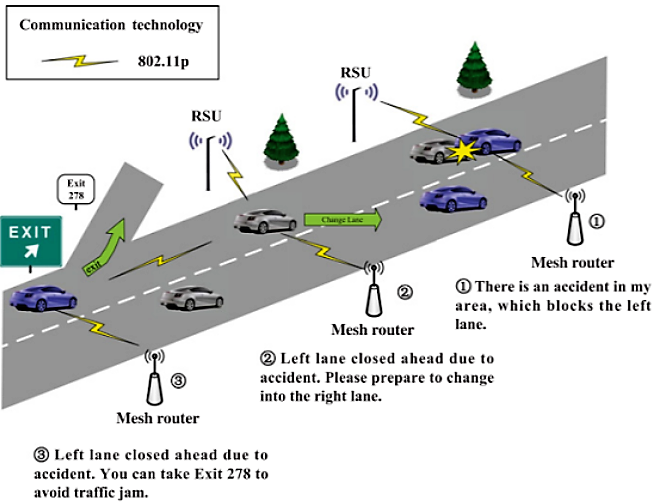
\includegraphics[scale = .49]{vanet.png}\\
\small{Figure 1 Vehicular Communication [11]}
\break
\end{center}

\subsection{Public Opinion}
In this paper we assume autonomy in ITS is accepted, and the public is willing to use an autonomous car as a mode of transportation. This happens when the public is confident that ITS “are safe from hacks, viruses, and other malicious elements that could cause widespread damage” [23]. Although we operate under the assumption that ITS will be accepted as a mode of transportation, it is clearly not the case now. (See figure 2). In recent years, more people have put their trust in semi-automated vehicle functions, and this trend has not yet been carried over into fully-automated functions.
\begin{center}
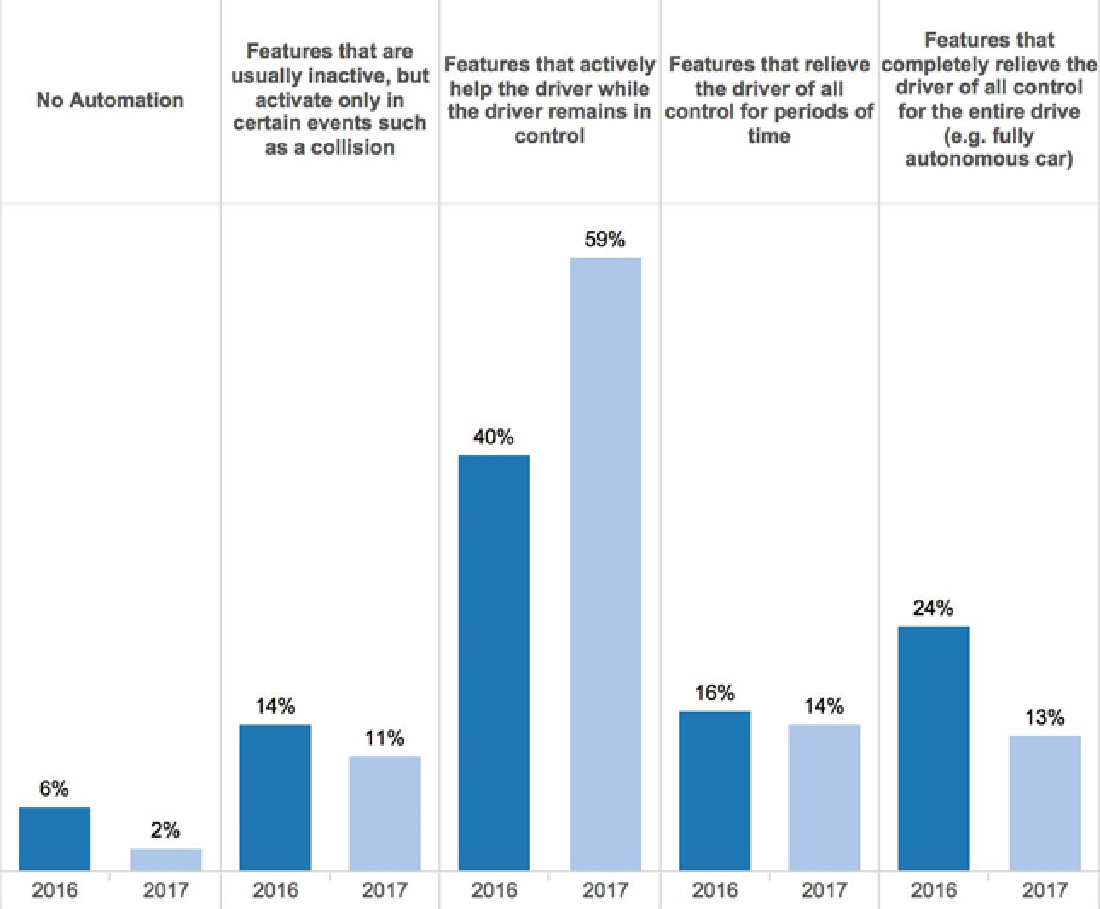
\includegraphics[scale = .3]{opinion.png}\\
\small{Figure 2 Public Automation Comfort Level\\ in 2016 and 2017 [1]}
\break
\end{center}
This is problematic, because if consumers do not adopt this new mode of transportation, the benefits of vehicular communication will not be experienced. An important contributing factor towards achieving public acceptance in ITS is how secure and private consumers consider autonomous vehicles to be. Recent surveys have indicated that one half of consumers do not consider their information secured [23], and new car buyers are increasingly concerned that car connectivity will put them at risk for hacking without meeting this expectation autonomous technology will fail [23]. This research however, will contribute to continue to increase public trust in ITS.

\subsection{Thesis}
Connected autonomous cars, ITS, there are many names for what is arguably the biggest revolutionary technological advance in recent history. Many different companies and universities are racing against the clock to become the first to successfully implement this technology. The two following sections will analyze two critical software attributes of ITS: security and privacy. This paper will define the best proactive security schemes and privacy protocols in ITS as an antecedent to a time when these vehicles will become fully connected and automated. 

%%%%%%%%%%%%%%%%%%%%%%%%%%%%%%%%%%%%%%%%%%%%%%%%%%%%%%%%%%%%%%%%%%%%%%%%%%%%%%%%%%%%%%%%%%%%%%%%%%%%%%%%%%%%%

\section{Security in ITS}
Communication between ITS cars over a vehicular ad hoc network (VANET) can reduce traffic, create more efficient roadways, and even potentially save lives. However, the introduction of this communication network, while beneficial, opens a myriad of attack vectors in which an adversary can attempt to cause harm. Malicious actors can sit between two vehicles, or nodes, and prevent communication, eavesdrop on the messages being sent, or alter the messages to send their own commands to unwitting receivers. Therefore, when designing a secure communication scheme, especially one transmitting safety-critical information, it is important to consider the worst-case scenario to be true: that every message sent will have a sophisticated and high-resource attack leveled against it.

\subsection{Security Imperatives}
Between any two communicators, whether that be Alice and Bob chatting over the phone or two autonomous cars traveling on the highway at high speed, there will be an adversary between them, ready to intercept and alter their communications. This line of thinking requires security professionals to take certain imperatives under their consideration when designing a secure communication scheme, including: confidentiality, authentication, non-repudiation, and integrity. Confidentiality requires that the information flowing from the sender to the receiver should not be eavesdropped and that this information be obscured from malicious eyes. Authentication or accountability, a major requirement in communication networks, ensures that messages are sent only by legitimate senders and in turn the messages reach the intended recipient. Non-repudiation can be summed up as accountability. The term “repudiation” refers to the ability for any sender of a message to later deny that they did send that message. Therefore, non-repudiation as an imperative prevents users from performing this potentially treacherous act and ensures accountability. Lastly, integrity demands that the information sent is equivalent to the information received and that no messages are altered or dropped during transit.

\subsection{Secure Communication Fundamentals}
Many of these imperatives can be achieved by implementing a computationally secure cryptographic protocol, namely RSA, Elliptic Curve, or the promising Lattice-based cryptography. These cryptographic protocols can be used to encrypt messages, making them unreadable to anyone besides the sender, who encrypted the message in the first place, and the receiver, the only entity with the ability to easily decrypt the message. In all modern cryptographic protocols, the encryption and decryption processes uses keys, which are strings of bits generated pseudo-randomly and used as inputs in encryption/decryption algorithms along with the plaintext messages. An encryption algorithm $E()$, with inputs key $k$ and message $m$, can be represented as $E(k, m)$. This results in a ciphertext message $c$.

\begin{center}
\large $E(k, m) => c$
\break
\end{center}

To decrypt the ciphertext, all the receiver needs to do is reverse the encryption function and input the secret key again, along with ciphertext, i.e. $D(k, c)$ which results in the original plaintext message $m$.\\

\begin{center}
\large $D(k, c) => m$
\end{center}

\hfill [15]


\subsection{Computation Security and Confidentiality}
Kerckhoffs Principle is a cryptographic primitive which implies that it's essential to consider every that adversary is knowledgeable about everything involved with the encryption and decryption process, save for the secret key [15]. It's best not to rely on security via obscurity, wherein the process that performs the encryption is kept secret, but instead to rely upon the actual strength of the algorithm being implemented. Always assume the adversary can see the ciphertext traveling through the network and is aware of what cryptographic protocol is being used. While the idea of an adversary seeing the ciphertext is troubling, the only way to derive the plaintext message from the ciphertext is to perform the decryption operation, which requires the secret key. This means that when attempting to break a message’s encryption, the only recourse an adversary has is to attempt to guess the secret key being used. The security of a cryptographic protocol then depends on how well the secret key is kept hidden and just how many possible keys exist for the adversary to try. 

A cryptographic protocol with a reliable algorithm and a large key space can be referred to as computationally secure, that is, it will take an adversary an unreasonable amount of time to guess the proper key and decode the secret message and by then, whatever message was sent will be irrelevant. The lengths of these keys and the process through which they're generated varies from algorithm to algorithm, but it's the use of these keys that partially satisfies the imperative of confidentiality. Again, confidentiality is the concern of keeping secret information private and the use of secret keys ensures that only those who know the applicable key can perform the decryption process [24].

\subsection{Cryptographic  Communication Schemes}
\subsubsection{Symmetric vs. Asymmetric}
Up to now, only one key has been referred to and used both in the encryption and decryption process. In cases where there is only one secret key, the cryptographic scheme can be referred to as a symmetric scheme, as each party has access to the same information [15]. However, establishing that secret key over an unsecure channel, between two parties that have never met face-to-face is difficult and symmetric schemes do not always satisfy all imperatives; in such cases, an asymmetric scheme is preferable.

In an asymmetric scheme, every user that wishes to communicate must generate for themselves a pair of keys, a private-key that is kept hidden and a second, public-key, that will be known to everyone [14]. For instance, autonomous car $A$ shall have: $a-$ and $a+$, private and public-key respectively, and autonomous car $B$ will have its own pair of keys: $b-$ and $b+$. To encrypt a message $m$, using encryption algorithm $E()$, to communicate with car $B$, car $A$ would first retrieve car $B$'s public-key and input that into the encryption algorithm with the message.\\

\begin{center}
\large $E(b+, m) => c$ 
\break
\end{center}

The relationship between any two public and private-key pair is such that when car $B$ receives the ciphertext, car $B$ can decrypt the ciphertext using its own private-key that no one else has access to.\\

\begin{center}
\large $D(b-, c) => m$
\end{center}


\subsubsection{Authentication and Non-Repudiation}
Asymmetric cryptography is widely used today in online communications, where parties wishing to communicate securely have never previously met face-to-face. This is possible because public-keys are kept on an online database referred to as a key repository, such as \emph{pgp.mit.edu} or \emph{pgp.key-server.io}. Users that generate their key pairs can post their public-key to these repositories for free, allowing anyone that wishes to communicate securely to send them messages only they can decrypt [15]. This functions as a form of receiver authentication. Say an entity, named \emph{Alice}, encrypts a message with a public-key belonging to another entity, named \emph{Bob}, then \emph{Alice} can know without a doubt, that \emph{Bob} will be the only entity able to decrypt it, since only \emph{Bob} knows his private-key. 

Achieving sender authentication, on the other hand, requires more finesse. Without a doubt, it is important for \emph{Bob} to know if the message they have received is really from the appropriate sender. A malicious adversary can just as easily encrypt a message with \emph{Bob’s} public-key and send him a message, while impersonating \emph{Alice}. To authenticate herself, \emph{Alice} must sign her message with a digital signature that is  unique to her; namely her private-key. This is possible by re-encrypting her cipher $c$ and her private-key $a-$ with the encryption algorithm $S()$ to produce the final payload:\\

\begin{center}
\large $S(a-, c) => payload$ 
\break
\end{center}

Upon receiving the payload, \emph{Bob} can reverse that function to verify \emph{Alice’s} signature using her universally known public-key: $V(a+, c)$; after which, he can decrypt the ciphertext normally to derive the original plaintext [15].\\

\begin{center}
\large $S(a-, E(b+, m)) => payload = > V(a+, D(b-, m))$ 
\break
\end{center}

Through this process, any user can authenticate themselves to the entity they are communicating with, and all payloads transmitted are unequivocally tied back to the original sender and owner of the private-key [24]. This satisfies not only the imperative of authentication, but also the imperative of non-repudiation. In ITS communication, where nodes have the potential of sending safety-critical information, messages that give false information and wreak havoc, intentionally or not, must be traced back to the sender so that an investigation can be conducted [24]. This Digital Signature Protocol provides an accountability not found in a symmetric scheme. However, the added step of signing a message does increase the computational overhead; meaning that in general, an asymmetric communication scheme performs slower than a symmetric communication scheme [15].

\subsubsection{Integrity and Hash Functions}
Integrity checks can also increase overhead, although it’s a necessary step to ensure messages are not altered or corrupted via transit [24]. There is little in the way of preventative measures that can be implemented reliably to ensure integrity, since under Kerckhoff's principle the assumption is that only the key is hidden from the ever-present adversary. It is possible for malicious actors to position themselves between autonomous cars, acting as network nodes, and flip bits at random to corrupt messages. This is a low-level, but potentially harmful attack. Luckily, there are procedures that can be enacted to check if integrity has been compromised. A hash function is a one-way, compression function that maps any input of bits into a unique, fixed-length, output. A good hash function will be irreversible, have a large output space, and ensure that any changes made in the input string will have an avalanche effect, resulting in a wildly different output. Inputting a message payload into a hash function, $H()$, results in an output hash $h_1$. By attaching this hash to the payload before transmission, the receiver can input the message payload into the hash function again, to output hash$h_2$, and compare the two hashes $h_1$ and $h_2$ to see if they match. Any difference in the hashes will mean that the message has been altered during transit. If:\\
\begin{center}
\large $H(payload) => h_1 \neq H(payload) => h_2$
\break
\end{center}
then message has been compromised. By comparing the two hashes to see if they match, a receiver can check if the message has maintained its integrity while traveling over the unsecured channel [15]. 

All the imperatives addressed previously contribute towards building a secure cryptographic scheme. The tenants of confidentiality, authentication, non-repudiation, and integrity are all implemented in online communication today and autonomous cars will undoubtedly also require schemes that achieve these imperatives as reliably as possible. These schemes will consist of cryptographic protocols, key exchange procedures, digital signature algorithms, hash functions, and infrastructure to support the network. 

\subsection{Cryptographic Protocols}
Possible candidates for cryptographic protocols include RSA and Elliptic Curve.

\subsubsection{RSA}
RSA is the most popular public-key cryptosystem currently in use. Realized in 1977 by its inventors, Rivest, Shamir, and Adleman, the difficulty of RSA lies in its key generation. Without going too in-depth into the mathematics, each user computes a modulus $n$, which is the product of large prime numbers: $p$ and $q$, and randomly generates an integer $e$. With those in hand, another integer $d$ can be derived such that:\\

\begin{center}
\large $e * d \equiv 1~ modulo~ (p-1)(q-1)$
\break
\end{center}

As with typical asymmetric schemes discussed above, the modulus $n$ and integer $e$ are made public while integer $d$ is kept private, thus forming a private and public-key pair. If entity \emph{Alice} wants to encrypt a message $m$ to send to entity \emph{Bob}, she would perform the following operation:\\

\begin{center}
\large $m^e~ modulo~ n$ 
\break
\end{center}

Where $e$ and $n$ are \emph{Bob’s} public-key. After receiving the message, \emph{Bob} can decrypt with his private-key, integer $d$:\\

\begin{center}
\large $c^d~ modulo~ n$
\end {center}

\hfill [15]
\break

The mathematical process necessary for key generation means that RSA is relatively slow [15]. However, RSA is among the most merited and time-tested encryption protocols since it is generally considered to be near impossible to determine the prime factors of a very large number, other than by brute-force, in polynomial time. This implies that it will take an adversary an unrealistic amount of time or computing power to factor the public modulus $n$ to find $p$ and $q$ and then derive the private integer $d$ [21].


\subsubsection{ECC}
Elliptic Curve Cryptography (ECC), while ostensibly more complicated, does pose certain advantages over RSA. Elliptic curves are based off modular arithmetic in which operations provide answers that are circular; in other words, the numbers in a finite field are limited and wrap around when the output of an operation exceeds their limits. For example, a finite field of order $7$ would consist of integers $\{0, 1, 2, 3, 4, 5, 6\}$ and $modulus~ 7$ will only ever give answers within that field. To be considered a finite field, properties such as associativity, commutativity, closure, existence of an identity and inverses must be satisfied. The formula for a curve under which the field will be implemented must also be safely and extensively defined [7]. Many safe curves are variations on the equation:\\

\begin{center}
\large $y^2~ = ~x^3~ +~ ax~ +~ b$
\break
\end{center} 

Where typically the variables $a$ and $b$ are very large prime integers. Since most standardized curves are too large to be represented succinctly, for the purposes of explaining field arithmetic over elliptic curves, reference the graph below:
\begin{center}
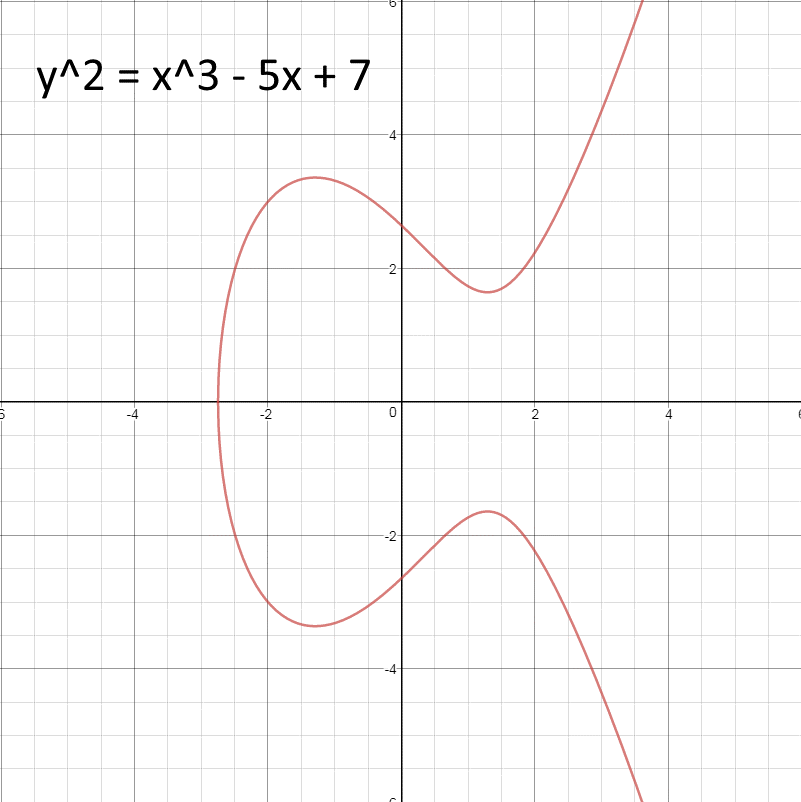
\includegraphics[scale = .385]{graph1.png}
\small {Figure 3 Elliptic Curve}
\break
\end{center}
To create keys for use in an asymmetric communication scheme, the user’s intent on communicating, entities \emph{Alice} and \emph{Bob} for instance, must first agree on a public curve. Parties performing operations with different curves will not be able to communicate with each other, forcing curves to be strictly standardized. Key generation can be performed through different methods, but for the purposes of this paper, an operation referred to as \emph{point dotting} via a scalar will be examined. \emph{Dotting} refers to a unique operation associated with a finite field, not quite addition and not quite multiplication, dotting, when applied to an element of a finite field, can return other elements in the field. To perform a dot operation, \emph{Alice} starts by selecting a point on the elliptic curve $P$. By drawing a line that intersects the elliptic curve tangentially at point $P$, \emph{Alice’s} line will intersect the elliptic curve again at another point, hereby referred to as $2P$. Since an elliptic curve is geometrically-symmetric around the x-axis, reflecting $2P$ over the x-axis will result in a third point $-2P$. Arriving at $-2P$ constitutes one dot operation over the finite field associated with the curve.
\begin{center}
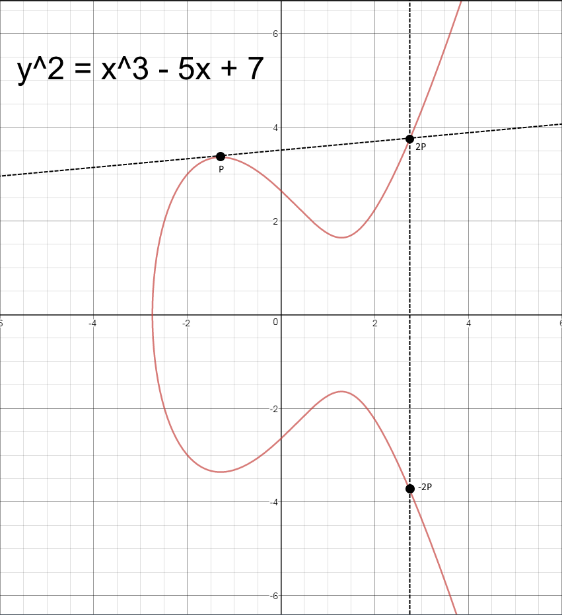
\includegraphics[scale = .515]{graph2.png}
\small {Figure 4 Dot Operation}
\break
\end{center}
Drawing a line from $-2P$ back to the original $P$ will cause the line to intersect with the elliptic curve at another point, $-3P$; reflecting $-3P$ over the x-axis will result in $3P$ - finishing another dot operation.
\begin{center}
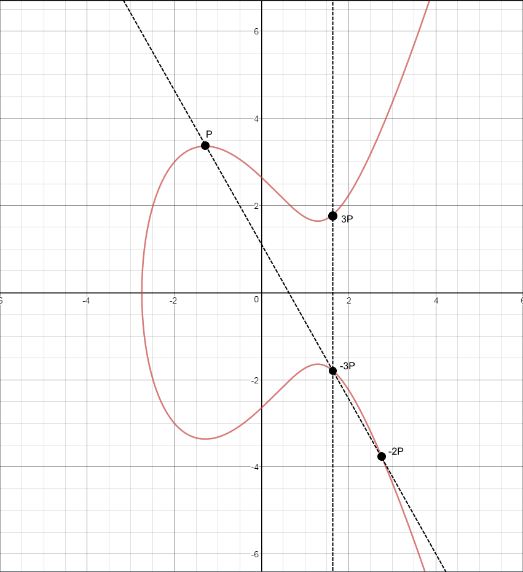
\includegraphics[scale = .54]{graph3.png}
\break
\small{Figure 5 X-Axis Reflection}
\break
\end{center}
This process is repeated, resulting in new $d_a*P$ points every time, where $d_a$ is the scalar integer applied to point $P$. Eventually, \emph{Alice} will arrive at a new point on the elliptic curve: $Q_a$, equal to $d_a*P$, which is her public-key. The scalar $d_a$ is kept secret and serves as \emph{Alice’s} private-key.\\

\begin{center}
\large $Q_a~ =~ d_a*P$
\break
\end{center}

Deriving the private-key, $d_a$, from the public components, points on the Elliptic curve $Qa$ and $P$, is referred to as the \emph{Elliptic Curve Discrete Logarithm Problem} (ECDLP):\\

\begin{center}
\large $d_a~ =~ log_pQ_a$
\end{center}

\hfill[15]\\

As of today, the computations required to brute-force the ECDLP is on average $n/2$; meaning that any key over 160 bits will result in an ECDLP that is computationally infeasible, as an adversary will on average must try 280 permutations. That said, the controversy around Elliptic Curve Cryptography stems, in part, from the uncertainty that an efficient algorithm for solving the ECDLP does or does not exist. The cryptographic community is hesitant to risk encrypting data with a protocol which may be proven to be easily broken in the next few years when a mathematical wizard publishes a new proof. The likelihood of this is low, however, as such a proof would imply the complexity class of a decision (yes/no) problem with polynomial-time algorithms is different than the complexity class of decision problems whose “yes” answers can be verified in polynomial-time if one is presented with an appropriate proof. Whether the complexity class of decision problems with polynomial-time algorithms is equal to the complexity class of problems is one of the outstanding open-ended questions in computer science [7].

\subsubsection{RSA vs. ECC}
Comparing Elliptic Curve Cryptography to RSA, Elliptic Curve is the most prudent regarding securing communication in ITS. Why Elliptic Curves though? The key generation, while interesting to visualize, appears to be more computationally time-consuming than RSA key-generation, especially considering the ‘dot’ operation will need to be performed potentially millions of times. Also, the strict standardization of curves leaves little room for variation in implementation, not to mention the possibility that some curves may be designed poorly and come with built-in backdoors. RSA is time-tested and widely accepted as being resistant to most adversary attacks, in addition, it’s removed from the controversy surrounding the mathematical basis of its development.

All that said, regarding encrypting communication in autonomous cars, Elliptic Curve is undoubtedly the cryptographic protocol best suited for their specific needs. Traveling at high speeds, ferrying people for miles, sending safety-critical information, navigating around other cars and obstacles, every computation counts, and the amount of time wasted on overhead can be life or death. While the key generation process may be time-consuming for Elliptic Curves, the final output is an incredibly secure key with a stunningly short length. Elliptic Curve keys of length 256 bits provide the same security as RSA keys over 3,000 bits in length [7].
\begin{center}
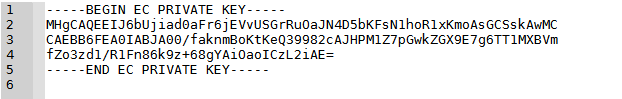
\includegraphics[scale = .58]{ecc.png}
\small {Figure 6 ECC Private-Key\footnote{256 bits, generated in OpenSSL}}
\break
\end{center}
\begin{center}
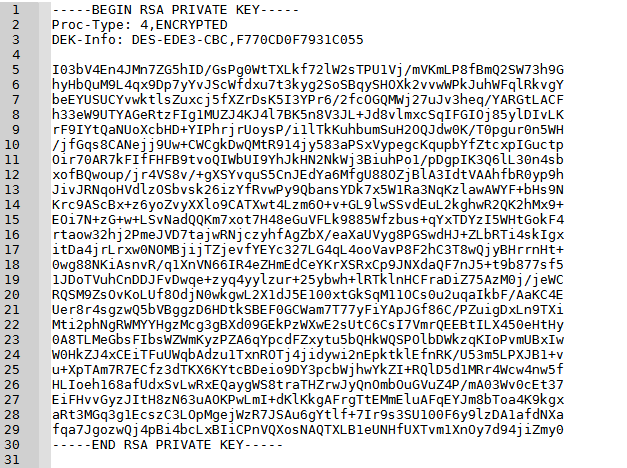
\includegraphics[scale = .58]{rsa.png}
\small{Figure 7 RSA Private-Key\footnote{2048 bits, generated in OpenSSL}}
\break
\end{center}
Shorter key sizes mean that more key-operations, signing with Digital Signatures and encryption/decryption, can be processed per second. Faster processing means messages arrive faster, allowing ITS to communicate as often as necessary and not waste as much computing power on cryptographic arithmetic. This moderate approach reduces the memory storage and bandwidth required as well, making the whole system more efficient [7].

\subsection{Proposals}
\subsubsection{Cryptographic Proposal}
The United States Federal Communications Commission (FCC) has already allocated a Dedicated Short-Range Communication (DSRC) spectrum for V2V and V2I communication, 75 MHz (5.85 - 5.925 GHz) in the 5.9 GHz band, laying down the groundwork for the VANET autonomous cars will be using soon [24]. To secure this communication channel, a hybrid symmetric/asymmetric scheme is most prudent, utilizing Elliptic Curve Integrated Encryption Scheme (ECIES) to establish communication between nodes using private/public-keys. ECIES, proposed by Bellare and Rogaway, is based off a previous public-key encryption scheme, ElGamal, and functions as a symmetric/asymmetric hybrid scheme [7]. Under ECIES, if Bob wishes to send a message to Alice, he would need to perform the following operations:\\
\break
\indent 1)~Generate a random integer $r$ between $0$ \footnote{With a key length such as 256 bits.}\\ %%%%need to find correct symbol for dot multiply
\indent 2)~Dot-multiply $r *$ point $P$ to produce a new point $J$\\ 
\indent 3)~Dot-multiply $r * Q_a$ \footnote{Alice’s public-key} to get point $S$ \footnote{Symmetric Key}\\

\hfill [7]\\

To encrypt his message, \emph{Bob} will utilize a block cipher, preferably the \emph{Advanced Encryption Standard} (AES). The use of a block cipher for encryption give ECIES the speed it needs for real-time applications. \emph{Bob} then will send his ciphertext and coordinates of point $J$ to \emph{Alice}. Upon receiving the payload, \emph{Alice} will derive $J$ with her private-key. Since the components of $J$ are $r * P$, \emph{Alice} can easily derive $S$ by multiplying it with her private key $d_a$:\\

\begin{center}
\large $S = J * d_a$\\ $=> S = r * P * d_a$ \\ $=> S = r * Q_a$
\break
\end{center}

Since $d_a * P$ is equivalent to $Q_a$, it follows that $Q_a * r$ will return the secret key $S$ [7].

Other encryption protocols exit with different curves and parameters. However, ECIES is the only asymmetric encryption algorithm, along with the \emph{brainpoolP256r1} curve, specified in the IEEE 1609.2 standard, which proposes security standards for V2V and V2I communication [18]). The \emph{brainpoolP256r1} curve as specified in RFC 5639 is defined under the equation:\\

\begin{center}
\large $y^2~ =~ x^3~ +~ (a~*~x)~ +~ b~ modulo~ p$
\newpage
\end{center}
With parameters\footnote{Represented in Hexadecimal}:\\
\begin{center}
$a$ = 7D5A0975FC2C3057EEF67530417AFFE7FB8055C\end{center}

126DC5C6CE94A4B44F330B5D9
\begin{center}
$b$ = 26DC5C6CE94A4B44F330B5D9BBD77CBF958416\end{center}

295CF7E1CE6BCCDC18FF8C07B6
\begin{center}
$p$ = A9FB57DBA1EEA9BC3E660A909D838D726E3BF6\end{center}

23D52620282013481D1F6E5377

\hfill{[12]}\\

After verifying if nodes are legitimate, all further encryption/decryption will use a session key through AES-256-GCM, see figure 8.
\begin{center}
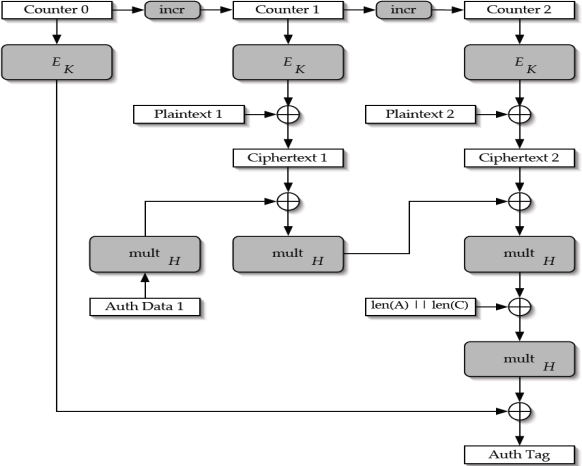
\includegraphics[scale = .55]{aes.png}
\small {Figure 8 AES-GCM Algorithm [2]}
\break
\end{center}
AES is a NIST endorsed block cipher based off the Rijndael cipher developed by Belgium cryptographers Daemen and Rijmen [15]. Block ciphers operate by parsing messages into fixed-length blocks, 128-bits in AES, and encrypting each block one at a time. While a multitude of different encryption modes exist for AES - EBC, CBC, CFB, and OFB to name a few - Galois/Counter Mode (GCM) is the superior choice as its functionality is such that both encryption and decryption can be performed in parallel. Parallel encryption/decryption means that multiple blocks of the message can be encrypted/decrypted at the same time, greatly improving speed. Other encryption modes require blocks to be decrypted in a specific order, which can increase overhead. Although IEEE 1609.2 proposes the use of AES-128-CCM, AES-256 provides greater security due to the longer key-length and GCM provides a built-in authentication checksum not found in CCM [18]. This means AES-256-GCM is highly optimized for authentication of the resulting ciphertext produce from encryption, which, in conjunction with a traditional hash function, can be used to ensure the integrity of messages before and after transit. Thus confidentiality, sender authentication, and message integrity are assured via ECIES with AES-256-GCM [5].

General authentication and non-repudiation will require the use of digital signatures, which will be generated for each autonomous vehicle through the widely accepted Elliptic Curve Digital Signature Algorithm (ECDSA), which functions as follows:\\
\break
1) Generate random integer $k$ from \{1, …, n - 1\} (where

$n$ is the order of the group, say $2^{256}$)\\
2) Calculate the point $L~ =~ k~ *~ P$ (where $P$ is the base)\\
3) Calculate the number $r~ = ~xL modulo n$ (where $xL$ is 

the x-coordinate of $L$)\\
4) If $r = 0$, then return to step 1\\
5) Calculate $s ~= ~k~-~1~(~z ~+~ r~ *~ d_a~)$ mod $n$ (where 

$d_a$ is \emph{Alice'}s private key and $k-1$ is the multiplicative 

inverse of $k modulo n$).\\
6) If $s ~=~ 0$, return to step 1.\\
7) Output digital signature is a point on the curve $(r, s)$\\

\hfill{[7]}\\

These digital signatures generated via ECDSA will be a component of each vehicle’s Digital Certificate, which will be verified by roadside units before allowing a node access to the network. A Digital Certificate for an autonomous car will list the following information: the relevant information of the party who issued the certificate, including the issuer’s public-key, signature algorithm identifier, and hash function identifier; the relevant information of the recipient, including the recipient's public-key and key algorithm identifier; and the validity period of the certificate [15]. 

The Certificate Authorities who issues these Digital Certificates will have to be trusted third parties, namely Vehicle Inspection Stations. For ITS cars to be useable and allowed into the VANET, they will need to pass a vehicle inspection to make sure they’re safe to operate physically and software checks to ensure allowing the nodes access to the network won’t introduce bugs or viruses into the network. Only after they have been deemed safe will autonomous cars be awarded their Digital Certificate.

\subsubsection{Infrastructure Proposal}
The infrastructure needed to securely operate the VANET for autonomous cars is only speculative in nature, but Certificate Authorities (CA’s) and Road-side Units (RSU’s) are completely necessary. Nodes that misbehave will be held accountable through their Digital Signature while their Digital Certificate is revoked, disbarring them from re-accessing the VANET. As for the communication that occurs, the RSU’s will be essential in transmitting the messages between cars. While nodes will be able to communicate asymmetrically in certain situations, i.e. for broadcasted messages, such as route blockages and emergency situations, RSU’s will be able to reach every node in its radius that is symmetrically connected to them. Much like cell-towers used for phone communication, each RSU will have a unique, periodically refreshed, symmetric key used for communicating with nodes connected to the network within its radius. Only after verifying a node’s Digital Certificate, will the RSU and node perform a \emph{handshake} and use their public and private-key pairs to exchange the RSU’s symmetric key. As a node passes from one RSU’s radius and enters another, the first RSU will pass the node’s service to the second. Since the first RSU has already verified the identity of the node, the second RSU can exchange its symmetric key with the node without having to perform the initial \emph{handshake} again. How the message log and the information therein will be stored and handled is a matter of privacy and, while often considered an imperative of security, is in this case considered to be of equal importance. The information of the legitimate actors within the network, data that is collected periodically and frequently, should be protected from unauthorized observers.

\subsection{Rebuttal}
Critiques of the cryptographic proposal above may follow our assumptions - that in the near-future ITS will not only be socially acceptable, but feasible – to the logical conclusion that our modern cryptographic protocols and algorithms may be insufficient by then, in the face of commercially available quantum computers. This is possible thanks to \emph{qubits}\footnote{Known as quantum bits.} which refers to a superposition of the traditional bit, either a 1 or 0. Qubits can be represented as a linear combination, wherein for $n$ qubits, there are $2n$ different states for any quantum logic-gate and operations performed on them can be performed in parallel [9]. Essentially problems such as the ECDLP, which are hard for classical computers to solve faster than polynomial-time, can be solved much quicker with quantum computers. This would result in all cryptographic protocols currently implemented being rendered insecure. To combat this, quantum-resistant cryptographic protocols need to be developed, the most promising of which circulating cryptographic journals now is referred to as Lattice-based cryptography. A lattice is defined as the set of all integer combinations of linearly independent vectors, referred to as a basis.
\begin{center}
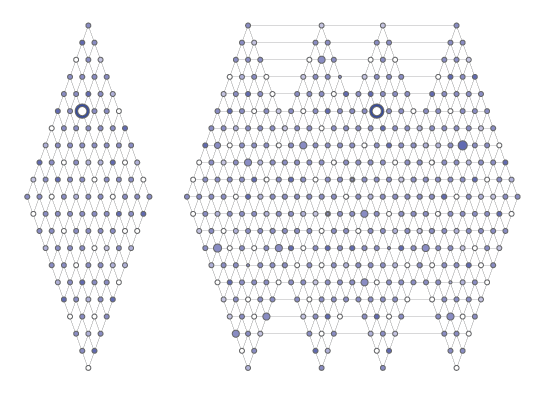
\includegraphics[scale = .6]{lattice.png}
\small{Figure 9 Lattice Cryptography [10]}
\break
\end{center}
The two main lattice problems that make Lattice-based cryptography so promising are the Shortest Vector Problem (SVP) and the Shortest Independent Vector Problem (SIVP), which can be used to formulate a public-key cryptosystem due to their hardness [19]. That said, while there currently exists no quantum algorithm to solve these problems quickly, it’s possible that one may come into fruition as quantum computers themselves become commercially available.

\subsection{Final Thoughts}
This section has introduced the fundamentals of secure communication, including encryption primitives using keys and Kerchoff’s principle, which regards the adversary of being knowledgeable about everything in the encryption process save for the secret key(s). The notion that all communication may be subject to an attack requires professionals to evaluate the security needs of ITS regarding their dedicated communication network and implement a secure cryptographic scheme. A hybrid symmetric/asymmetric scheme through ECIES with AES-256-GCM, in conjunction with ECDSA, is the most judicious option in comparison to other cryptographic protocols - due to the ECC’s speed and superior security. Although further research into cryptographic algorithms and development of autonomous cars may prove the need for more future-proof cryptographic protocols, the proposal above is the best current choice for securing communication in ITS.

%%%%%%%%%%%%%%%%%%%%%%%%%%%%%%%%%%%%%%%%%%%%%%%%%%%%%%%%%%%%%%%%%%%%%%%%%%%%%%%%%%%%%%%%%%%%%%%%%%%%%%%%%%%%%

\section{Privacy in ITS}

Autonomous cars can only be successfully implemented as a mode of transportation if they are considered safe, reliable, and trustworthy. Current research trends indicate that in the near future autonomous cars will have the capability of communicating with one another and relay important information, but little attention has been given to keep this exchange both private and secure. Therefore, the communication components in autonomous cars should be designed where the protocols for privacy should are explicitly established, and secure communication schemes defined. This paper will analyze the importance of ensuring the requirements for both privacy and security are equally addressed. 

\subsection{Background and Expectations}
Privacy is traditionally defined as a requirement to security. This has led to a problematic hierarchical representation of system requirements, with security outranking privacy. This is not the correct approach, as in following it many privacy requirements are continuously overlooked. Privacy is equally as important as security, as both are important factors for public acceptance and successful deployment of a Vehicular Ad Hoc Network, or VANET [23].

The “entire ecosystem,” or the entire automotive industry, needs to work together to ensure the “physical and digital safety [and privacy] of drivers is prioritized, so vehicles [are] robust enough to stand up to hacking attempts and any further abuse of data” [23].

With connected ITS, there are several potentially sensitive and identifying data components which are inevitably transmitted back and forth through the VANET. Examples of collected data from a single vehicle, or node, include “time, location, vehicle identifier, technical description, [and] trip details” [24]. The collection of this data is important and useful because as connected cars communicate important information through the VANET, this will lead to better traffic conditions, accident prevention, and relevant infrastructure updates.

Moreover, as these connected cars are adopted as a mode of transportation, it is feasible that many vehicles will serve to transport an infinite number of passengers, as is common presently with ride sharing practices (Ride Sharing Programs). This will not only reduce accidents considerably, it will yield environmental benefits. However, every individual that becomes a passenger in a shared, connected autonomous car will have identifying personal information that inherently is collected and transmitted through the VANET. A connected car equipped with ride-sharing capabilities will collect data to include: “recent or favorite destinations, personal details on user, including payment details, preferences relating to seating, temperature, music, etc.” [23]. This data collection is inevitably associated with the risk of data “being mistakenly shared between users” [23].

Attention will have to be given to how this information is collected, stored, and shared through the VANET. Consumers will have high privacy expectations, especially given recent privacy violations, thus steps must be taken to protect their personal information. 

\subsection{Imperatives and Requirements}
The security imperatives, or requirements, previously discussed as they relate to data privacy include confidentiality, access control, and authentication. There are also fundamental “privacy by design” requirements that should be regarded when designing connected vehicles, to safeguard consumer privacy [23]. 

\subsubsection{Confidentiality}
To reiterate, confidentiality implies that information moving through the VANET “should not be eavesdropped” [23]. However, for the accountability security requirement to be satisfied, all identities cannot be kept completely anonymous. It is important however, that this requirement be given consideration, to avoid unnecessary linkage of information shared with sending nodes.

\subsubsection{Access Control}
Access control is the capability of distinguishing between access levels of a node or infrastructure component, “established through specific system-wide policies, which specifies what each node can do in the network” [24]. This requirement is important, as it determines how the system is compartmentalized. Doing this in a way that protects the consumer’s privacy can be tricky, and a practical approach will be later discussed

\subsubsection{Authentication}
Authentication, in terms of the lifetime of data, asserts that the information being transmitted is “fresh and live,” meaning the information is both sent and received within an acceptable time frame [24]. As a security requirement, authentication ensures an individual node can be given access to communicate within the VANET. As discussed, this is achieved by assigning digital certificates. However, as a privacy requirement, authentication should not jeopardize private information by linking the multiple digital certificates that one user accumulates.

\subsubsection{Transparency}
Transparency is crucial; consumers must be kept informed as to how their data is used. That is, the consumer should be aware of who has access to their data, and to what purpose this data is being used. This requirement should not be considered satisfied by having consumers sign long, complicated agreements prior to operating the system. This practice is wrong, and should be discontinued. As most of these agreements are worded in a way that most consumers do not understand and do not bother with reading. The most relevant terms should be openly shared with consumers. 

\subsubsection{Sovereignty}
The jurisdiction, or sovereignty, of how data is managed, in addition to risk management, should be awarded to the consumer and the company involved. This is important for two reasons. First, it is the parties involved that have the most relevant information for how a system should operate and be monitored. Allowing outside parties, with no knowledge of the system requirements and applications, to intervene would introduce superfluous and potentially damaging practices. Secondly, the parties most affected by the system vulnerabilities are the ones who have the most to lose. Therefore, their judgement should be sufficient and should be trusted.

\subsubsection{Value Added Purposes}
When considering how data will be shared with outside sources, the consumer should be well informed as to how this sharing will constitute a value-added purpose. In other words, there needs to be real value, to the consumer, resulting from the data sharing. For example, the consumer can be given the option to have their personal health record available in the connected autonomous vehicle, for use in emergencies. However, this data should only be made available to first responders, and other health professionals, who have been given relevant permissions. This health record, however, should not be accessible to “any non-medical party” [23]. This would be a good example of an added-value purpose, since the consumer would directly benefit from having their data shared with the health personnel who are facilitating live-saving measures.

\subsubsection{Data Minimization}
Data minimization, or minimum disclosure, entails reducing the amount of information collected only to the “data that is really needed for the application, and nothing else” [23]. This privacy requirement is common in many applications and is frequently referred to as need to know. This is both practical and necessary. Data minimization ensures that superfluous information is not collected and stored, slowing down safety-critical functions. Also, when sensitive information is either unintentionally disclosed or maliciously collected, it will make the process of identifying remedial measures less time consuming.

\subsection{Privacy Protocols}
What follows will serve to discuss three specific privacy schemes, or protocols, that can be implemented to enhance user’s privacy in a connected ITS. 

\subsubsection{Conditionally Confidential Approach}
To avoid issues arising with erroneous data transmissions, some have proposed that data transmissions remain conditionally confidential. 

One way of achieving this would be that senders of relevant information remain anonymous to the connected vehicles that are receiving their transmissions. These senders, however, would be traceable by a third party, the certificate authority (CA), presumably through the infrastructure system [24]. The CA would then could retrieve the identity of the sender if needed. This would satisfy the non-repudiation privacy and safety requirement, but it is uncertain if the confidentiality requirement would be satisfied. Confidentiality would be reasonably maintained, but it would be necessary to ensure the CA is protected from adversaries. It would also be necessary to ensure the CA itself does not have the ability to use this information with malicious intentions.

\subsubsection{Anonymous Data Set}
Another way to achieve confidentiality would be to create an anonymous data set. For all messages, $m$, transmitted within the VANET, there would exist a function, $f(m)$. \\

\begin {center}
\large $f(m) = m_k$
\break
\end {center} 

For all messages, $m$, there exists an information set, $k$, such that $m_k$ represents connected autonomous vehicular communication.\\

\begin {center}
\large  $\forall$  $ m$ $\exists$ $ k:$
\break
\end {center}
\begin {center}
\large $f(m) = m_k$
\break
\end {center}

While a node represents a connected autonomous car in communicating through the VANET, $n_x$, and is an element of $k$, but is not in $f(m)$:\\

\begin {center}
\large $[$ ($n_x$ $\in$ $k$$)$ $\cup$ $(n_x$ $\notin$ $f(m) $) $].$
\break
\end {center}

This distinction is necessary to further satisfy the confidentiality requirement, as there would not be a possibility for the individual nodes to be linked with the messages sent. This is essential to prevent adversaries from “connecting the dots” and tracing the message to a node and then tracing that node to the individual in the connected vehicle. Subsequently, $n_x$ will represent all the nodes that could have reasonably sent the message, $m$, but does not include all nodes, $U$\footnote{$U$ is the universal data set containing all nodes, $n$, communicating within the VANET.}, hence:\\

\begin {center}
\large $In$ $ n_x $ $(U \neq x).$
\break
\end {center}

Therefore,\\

\begin {center}
\large  $For$ $ m_k;$ $ k =\{ n_1, n_2, n_3, ..., n_x\}.$
\break
\end {center}

Here the number of vehicles included in x would have to be extensive enough to prevent adversaries from guessing the true sending node. Relevant parameters would need to be established and randomized to prevent a threat.


\subsubsection{Distribution of Authority Approach}
A different privacy protocol, which can be implemented in parallel to others, is useful in preventing oversight by distributing power – that is who holds what information – amongst various entities, such as Certificate Authorities (CA) and others. The different groups would need to have fully disclosed their interest, and the groups should have “different intrinsic interests” [20]. 

Determining what authority is given to which company will be dependent upon the companies interests and capabilities. For example, it would not be possible to allow a marketing agency to be privy to consumer’s spending habits, as this will create a conflict of interest that could be damaging in terms of protecting privacy. 

A different privacy protocol, which can be implemented in parallel to others, is useful in preventing oversight by distributing power amongst various entities such as Certificate Authorities (CA). The different groups would need to have fully disclosed their interest, and the groups should have “different intrinsic interests” [20]. 
The separation of authority has clear benefits. It allows for the various entities to check one another in both the nature of their involvement and to ensure full protection by not giving one entity full disclosure of a node’s identity. The downfall would be that the additional involvement of different entities could result in errors and information corruption on various levels. 

There would need to be very clear and transferrable guidelines to avoid collusion or mistakes. This distributive approach also requires significant collaboration between the various CA, which is obvious, but not always easy to achieve. Problems could arise resulting from unclear expectations or lack of defining who has authority, or jurisdiction, over every specific component of the system.


\subsection{Scenarios and Risks}
Soon vehicles will undergo a revolutionary transformation. They will cease to be used solely for transportation, and will become a “personalized mobile information hub – fully connected to the outside world” [23]. Each vehicle is a node, communicating through the VANET, and each “transaction” of data sent or received from the infrastructure is recorded, and can be shared with other nodes, when relevant information is available. This, as previously discussed, poses a privacy risk. It is important to identify how the information collected is used and classify it as acceptable and non-acceptable uses.

\subsubsection{Acceptable Uses}
There are many ways in which data collected can prove useful. For example, insurance companies will have the ability to tailor their policies to the “personal driving behavior or [their] drivers” [23]. There are circumstances in which unbiased, reputable data needs to be accessed. 

For example, in the case of a criminal investigation, a court of law may need to obtain data concerning a traffic violation to determine a driver’s guilt or innocence. It is very likely that peace officers will be taken out of the equation altogether, since our cars will have the capability of regulating speed to ensure safety and efficiency.

Collisions, unfortunately will likely never be eliminated, if there is room for human error, so when a collision occurs, the data collected leading up to the crash will prove useful during collision analysis. This data can be used to assign culpability and provide feedback to both the driver and the automation engineers. 

Cell phone triangulation allows investigators to locate a criminal by tracking his cell phone, from the cell towers in the phone’s vicinity. Assuming autonomous cars will communicate using roadside units (RSU’s), much like cell phones are connected to cell towers, investigators will be able to triangulate a vehicle’s location. RSU’s will have a set radius where they provide service. As a car passes out of one RSU’s radius and enters another, a “hand-off” procedure is initiated wherein the car’s connection is passed from one RSU to another. 

This process will allow investigators to not only track a car’s path, but predict its trajectory. If a car is stationary in an urban area, it’s likely the car will be in the radius of multiple RSU’s at once. Investigators can use the RSU’s to approximate the distance between the car and the RSU, compared to other RSU’s, and thus locate the car. Figure 1 gives a visual representation of how three RSUs in one area would overlap the coverage they provide.\\
\begin{center}
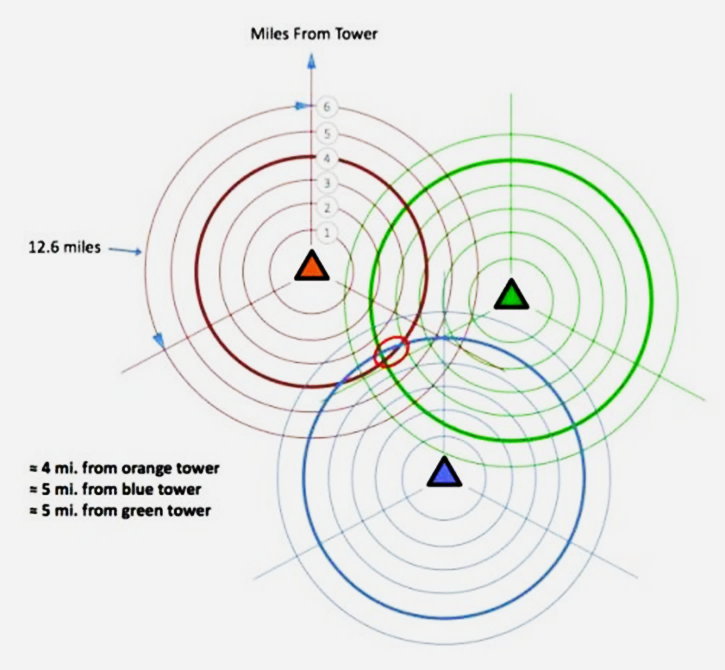
\includegraphics[scale = .98]{cell.png}
\small{Figure 10 Cell Triangulation [13]}
\break
\end{center}
The same concept could be applied to triangulate a vehicle’s location, if it is within range of a RSU. This application, however, must be carefully designed to allow vehicle location to only be accessed by law enforcement officials. Otherwise, this use could easily be exploited by an attacker to locate a vehicle in the network. 

\subsubsection{Non Acceptable Uses}
A consumer should be assured that steps are taken, in the design of connected vehicles, that will ensure unacceptable uses of their data are never encountered.\footnote{"“Privacy preservation is an important design requirement for VANETs, where the source privacy of safety messages is envisioned to emerge as a key security issue because some privacy-sensitive information, such as the driver’s name, license plate, vehicle model, position, and driving route, could be intentionally de-privatized so that the personal privacy of the driver is jeopardized" [24].}

Recent publicized information regarding data sharing on social media has angered consumers and made them question who has access to their information. 

Recent studies have also shown that “half of all internet users do not regard their data as secure on the internet” [23]. 

In the case of ITS, access to the internet of things implies data is collected and eventually driver preferences and frequently visited locations can be determined. This may be of great interest to advertising agencies, but the question arises: should this data be shared for the advantage of these companies? 

Many would feel this is a violation of privacy. Even when marketing agencies, working on behalf of a company, wish to exploit the information that is collected detailing a consumer’s personal preferences, further consideration must be given on whether this will be allowed under certain circumstances. 

For example, on the occasion that a customer opts-in, or when a free-trial of a ride-sharing automated vehicle is offered, a marketing company would be given limited access to the customer’s data.

\subsubsection{Privacy Threats}
It is not possible to plan for every different possible privacy threat that can occur, much like it is not possible to completely guarantee security, but there are various examples of how privacy can be violated that illustrate the importance of meeting privacy requirements. Here are a two possible privacy threats to consider when accounting for the various possible points of attack. \\
\emph{1) \indent Personal Information Leakage}\\
\indent This happens when information is transmitted over the VANET, if left unprotected, this information would be susceptible to discoverability by an adversary. Sensitive information, such as name, address, and license would be revealed, this constituting a privacy breach that could result in identity theft.\\
\emph{2) \indent Location Privacy or Eavesdropping}\\
\indent An adversary can intercept a significant number of messages in a certain region, the adversary may be able to trace a vehicle in terms of its physical position and moving patterns simply through information analysis.

\subsection{Proposal}
\subsubsection{Equal Importance}
As previously stated, privacy requirements are routinely overlooked. This is not an intentional failure in software design, but can most likely be attributed to the level of priority that is assigned to privacy as a software attribute. To reduce the risk of systematic oversight a change in methodology and processes is necessary. 

It cannot be overstated that security and privacy are both equally important and each have several requirements that are a subset to each, but are applied in different ways for each attribute. Figure 2 illustrates this notion.

This figure illustrates three key concepts. First, and most importantly, as this chapter has highlighted, privacy and security are both important and complex quality attributes of Intelligent Transportation Systems (ITS). This ideology is the most controversial proposal presented in this chapter, as is other systems privacy is categorized as a system requirement to security. Adding another “line item” in a budget creates concerns, and is most likely why many privacy requirements are ignored. 

Another important observation is that privacy and security are interdependent. This is denoted by the red arrows going back and forth from the two attributes. Several privacy requirements depend on security requirements, and several privacy requirements help achieve security goals. Furthermore, a system cannot be considered secure if it is not private, and the reverse is also true. 
\begin{center}
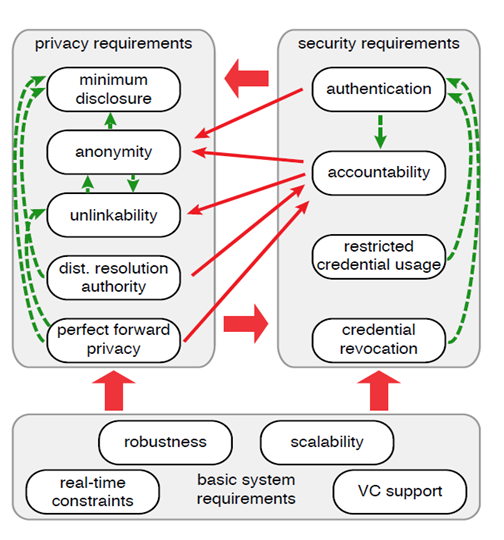
\includegraphics[scale = 1.05]{req.png}
\small{Figure 11 Requirement Mapping [20]}
\break
\end{center}
A third consideration is realizing the complexity of privacy, as a system attribute. It is clear how important it becomes to prioritize satisfying the requirements listed previously. If one is missed, the security of the system will be affected. This also illustrates how overlooking privacy requirements, as has continually happened, can be catastrophic. 

\subsubsection{Multi-Layer Approach}
It goes without saying that the more secure a system, the more consumers will trust and use the product. It is necessary to develop multi-layer security systems in today’s attack-prone world. A new source of revenue was created as hackers have learned to exploit system vulnerabilities, and one layer of protection is simply not enough. As discussed in chapter one, an asymmetric communication scheme can be used to encrypt and decrypt messages transmitted through the VANET. If this methodology is paired with the anonymous set, previously discussed in this section, a multi-layer protection scheme would satisfy both privacy and security requirements. Further, it would ensure that the system is more robust, and can withstand malicious attempts to infiltrate the system.

\subsection{Rebuttal}
The most common approach of securing a system has left privacy on the backburner, and most will argue that one is more important that the other. Because, how can a system’s requirements all be treated with equal importance? i.e. when everything is important, then nothing is. The truth is, many of the requirements in a system are vital in ensuring it is feasibly put on the market, so to speak, but some give and take must happen to protect the bottom line. The problem, then, is that in keeping with a company’s budget critical system requirements are overlooked, as has routinely occurred with privacy concerns. An argument should be made as to why the budget did not account for such critical line items as ensuring privacy to begin with. 
\subsection{Final Thoughts}
This section has highlighted the importance of achieving privacy requirements in the design of connected autonomous cars. Two privacy protocols, conditionally confidential and authority distribution, were also discussed. A proposal, including the notion that privacy is equally as important as security, was suggested. Connected autonomous cars will revolutionize traffic and transportation habits and by applying practical, systematic privacy protocols, the public will be guaranteed to accept this new form of transportation.

%%%%%%%%%%%%%%%%%%%%%%%%%%%%%%%%%%%%%%%%%%%%%%%%%%%%%%%%%%%%%%%%%%%%%%%%%%%%%%%%%%%%%%%%%%%%%%%%%%%%%%%%%%%%%

\section{Conclusion}
We have discussed two very important ITS requirements, security and privacy. In many ways, they depend on one another. As ITS become connected and communicate through a VANET, the systems will inevitably be exposed to considerable risks. To increase public trust in autonomous vehicles, both requirements need to be equally addressed in the design and development stages. ITS will revolutionize the way in which consumers view and use transportation services. 

To ensure that connected ITS can operate within the VANET both security and privacy requirements should be identified and met.	
To ensure that the communication network is considered secure, the security imperatives of confidentiality, authentication, non-repudiation, and integrity should be satisfied. This paper proposes the use of the Elliptic Curve Integrated Encryption Scheme (ECIES) because of its smaller key-size and superior security. AES-256-GCM is the encryption algorithm that provides the best balance of speed and security, due to its parallelism and built-in integrity check, required for the VANET. To generate digital signatures, for each node, the Elliptic Curve Digital Signature Algorithm (ESDSA) is proposed. For general-purpose integrity checks, and in use with pseudo-random functions, the checksum produced from hash function SHA-256 should be used. For important, broadcasted messages sent from Road-side units, a SHA-256 checksum can be appended to the message payload.
The privacy requirements, which need to be satisfied in ITS, are confidentiality, access control, authentication, transparency, sovereignty, value added purposes, and data minimization. In this paper, three privacy protocols were discussed; the conditionally confidential approach, the anonymous data set, and the distribution of authority approach. Two proposals were also presented, the equal importance proposal and multi-layer proposal. The most important consideration presented is that privacy requirements should be treated with the same amount of importance as security requirements. In ITS both attributes are interdependent on each other. 

Introducing connected ITS into the transportation system has the potential of making driving easier, more efficient, and generally safer [23]. By communicating with each other, ITS are capable of transmitting safety-critical information to other nodes, where that information can be processed, decisions made, and actions performed much quicker than with a human driver.  As stated previously, however, the notion of connecting the entire population of cars to a massive communication network, namely the VANET, and depending on that network to function safely, securely, and reliably is a gamble not many people are willing to take [23]. The fact of the matter is, the application of VANETS will give malicious adversaries many opportunities to cause harm and for the privacy of the cars owners to be violated due to the frequent collection of information that will occur [24]. 

To make VANETS secure and private, developers of the system must understand the communication fundamentals explained in sections one and two. However, as discussed in this paper, the security approach is only half the battle and developers routinely leave concepts such as privacy up to the discretion of corporations, who have proven themselves to devalue consumer’s interests. Therefore, it is sensible to value privacy as much as security and have well-defined privacy protocols that clearly express acceptable uses of data and protections for the identities of drivers.

Implementing the security and privacy proposals above may be the first step to making VANETS safe for use, thereby increasing that public trust. However, while the technology and infrastructure are being put into place for connected networks to operate feasibly, that reality is yet to come. Further research and development is required to match the advancements in technology that will undoubtedly come in the time when connected, fully autonomous cars come to fruition.

%%%%%%%%%%%%%%%%%%%%%%%%%%%%%%%%%%%%%%%%%%%%%%%%%%%%%%%%%%%%%%%%%%%%%%%%%%%%%%%%%%%%%%%%%%%%%%%%%%%%%%%%%%%%%

% use section* for acknowledgment
\ifCLASSOPTIONcompsoc
  % The Computer Society usually uses the plural form
\section*{Acknowledgments}

The authors would like to thank the National Science Foundation for it's support to undergraduate research, without whom this research could not have been possible, the Department of Computer Science at the University of Texas at Dallas, and other Research Experience for Undergraduates (REU) participants.  

\newpage

% references section

\begin{thebibliography}{1}

\bibitem{IEEEhowto:abraham}
Abraham, H.~, Reimer, B.~, Seppelt, B.~, Fitzgerald, C.~, Mehler, B.~, \& Coughlin, J. F. (2012). \emph{Consumer Interest in Automation: Preliminary Observations Exploring a Year's Change.} [Age Lab Life Tomorrow White Paper MIT]. Cambridge Massachusetts.

\bibitem{IEEEhowto:arun}
Arun, V.~, Vanisree, K.~, \& Reddy, D.~L.~ (2015). \emph{Implementation of AES-GCM encryption algorithm for high performance and low power architecture Using FPGA}.

\bibitem{IEEEhowto:chen}
Chen, L.~, Ji, J.~, \& Zhang, Z.~ (2013). emph{Wireless Network Security Theories and Applications.} Berlin, Heidelberg: Springer.

\bibitem{IEEEhowto:Definition of privacy}
Definition of Privacy. (2018, June 29). Retrieved July 11, 2018, from https://www.merriam-webster.com/dictionary/privacy

\bibitem{IEEEhowto:dworkin}
Dworkin, M.~ J.~ (2007). \emph{Recommendation for block cipher modes of operation}: NIST Special Publication 800-38D. doi:10.6028/nist.sp.800-38d

\bibitem{IEEEhowto:hadar}
Hadar, I.~, Hasson, T.~, Ayalon, O.~ et al. Empir Software Eng (2018) 23: 259. https://doi-org.libproxy.utdallas.edu/10.1007/s10664-017-9517-1

\bibitem{IEEEhowto:hankerson}
Hankerson, D.~, Vanstone, Scott A~, \& Menezes, A.~ J.~ (2004). \emph{Guide to elliptic curve cryptography} (Springer professional computing). New York: Springer.

\bibitem{IEEEhowto:haspiel}
Haspiel, J.~, Du, N.~, Meyerson, J.~, Jr.~, L.~ P.~, Tilbury, D.~, Yang, X.~ J.~, \& Pradhan, A.~ K.~ (2018). \emph{Explanations and Expectations: Trust Building in Automated Vehicles}. Companion of the 2018 ACM/IEEE International Conference on Human-Robot Interaction - HRI 18. doi:10.1145/3173386.3177057

\bibitem{IEEEhowto:bertels}
K.~ Bertels, \emph{Quantum computing: How far away is it?} 2015 International Conference on High Performance Computing \& Simulation (HPCS), Amsterdam, 2015, pp. 557-558. doi: 10.1109/HPCSim.2015.7237090

\bibitem{IEEEhowto:latice cryptography}
[Lattice Cryptography]. (n.d.). Retrieved July 11, 2018, from https://www.research.ibm.com/5-in-5/lattice-cryptography/

\bibitem{IEEEhowto:lin}
Lin, X.~, \& Lu, Rongxing. (2015). \emph{Vehicular ad hoc network security and privacy} (IEEE Press series on information \& communication networks security).

\bibitem{IEEEhowto:lochter}
Lochter, M.~ and J.~ Merkle, \emph{Elliptic Curve Cryptography (ECC) Brainpool Standard Curves and Curve Generation}, RFC 5639, DOI 10.17487/RFC5639, March 2010, <https://www.rfc-editor.org/info/rfc5639>.

\bibitem{IEEEhowto:locke}
Locke, P.~ (2012, June 1). [Image: Cell Tower Triangulation]. Retrieved June 12, 2018, from https://wrongfulconvictionsblog.org/2012/06/01/cell-tower-triangulation-how-it-works/

\bibitem{IEEEhowto:manvi}
Manvi, S.~, Kakkasageri, M.~, \& Adiga, D. (2009). \emph{Message Authentication in Vehicular Ad Hoc Networks: ECDSA Based Approach}. 2009 International Conference on Future Computer and Communication. doi:10.1109/icfcc.2009.120

\bibitem{IEEEhowto:mao}
Mao, W.~ (2004). \emph{Modern Cryptography: Theory and Practice}. Upper Saddle River, NJ: Hewlett-Packard Books: Walter Bruce.

\bibitem{IEEEhowto:marin}
Marin Perez, J.~ M.~, Juan, A.~ M.~, Perez, J.~ A.~, Rabadan, J.~ M.~, \& Skarmeta Gomez, A. F. (2015). \emph{Security and Privacy in Vehicular Communications with INTER-TRUST}. In Cyber Security and Privacy - 2015 (Vol. 4th, Cyber Security and Privacy Innovation Forum, pp. 53-64). Switzerland: Springer International Publishing. doi:10.1007/978-3-319-25360-2 5

\bibitem{IEEEhowto:maurer}
Maurer, M.~, Gerdes, J.~ C.~, Lenz, B.~, \& Winner, H.~ (2016). \emph{Autonomous driving: Technical, legal and social aspects}. Berlin: Springer Open. doi:10.1007/978-3-662-48847-8

\bibitem{IEEEhowto:mohammad}
Mohammad Khodaei, Hongyu Jin, Panagiotis Papadimitratos, \emph{SECMACE: Scalable and Robust Identity and Credential Management Infrastructure in Vehicular Communication Systems}, Intelligent Transportation Systems IEEE Transactions on, vol. 19, pp. 1430-1444, 2018, ISSN 1524-9050.

\bibitem{IEEEhowto:regev}
Regev, O.~ (2005). \emph{On lattices, learning with errors, random linear codes, and cryptography}. STOC.
Ride Sharing Programs. (2015, August 24). Retrieved July 6, 2018, from https://www.transportation.gov/mission/health/ride-sharing-programs

\bibitem{IEEEhowto:schaub}
Schaub, F.~, Ma, Z.~, \& Kargl, F.~ (2009). \emph{Privacy Requirements in Vehicular Communication Systems}. 2009 International Conference on Computational Science and Engineering, 139-145. doi:10.1109/cse.2009.135

\bibitem{IEEEhowto:stapko}
Stapko, T.~ J.~ (2008). emph{Practical embedded security building secure resource-constrained systems}. Amsterdam: Elsevier/Newnes.

\bibitem{IEEEhowto:The Regents of the University of Michigan}
The Regents of the University of Michigan. (2018). \emph{Leading the Transformation to Connected and Automated Vehicles: Our Work}. Retrieved July 10, 2018, from https://mcity.umich.edu/our-work/

\bibitem{IEEEhowto:watzenig}
Watzenig, D.~, \& Horn, M.~ (2017). emph{Automated Driving: Safer and More Efficient Future Driving}. Springer International Publishing Switzerland. doi:10.1007/978-3-319-31895-0

\bibitem{IEEEhowto:yang}
Yang, Weidong (2013). emph{Security in Vehicular Ad Hoc Networks (VANETs)}. In Wireless network security theories and applications (pp. 95 - 128)  (Springer ebooks : Computer science collection). Beijing: Heidelberg: Higher Education Press; Springer.

\end{thebibliography}

\end{document}


